\documentclass[aspectratio=169,12pt]{beamer}
% Estilo canónico para las presentaciones de Métodos Numéricos 2026-2.
\usepackage[T1]{fontenc}
\usepackage[utf8]{inputenc}
\usepackage[spanish,es-nodecimaldot]{babel}
\usepackage{lmodern}
\usepackage{amsmath,amssymb,mathtools}
\usepackage{booktabs}
\usepackage{graphicx}
\usepackage{xcolor}
\usepackage{hyperref}

\definecolor{upazul}{HTML}{003B70}
\definecolor{upazulclaro}{HTML}{EAF2F8}
\definecolor{updorado}{HTML}{C5962E}
\definecolor{upgris}{HTML}{4A5560}
\definecolor{upverde}{HTML}{167C5A}
\definecolor{uprojo}{HTML}{B33A3A}

\setbeamercolor{normal text}{fg=black,bg=white}
\setbeamercolor{structure}{fg=upazul}
\setbeamercolor{frametitle}{fg=white,bg=upazul}
\setbeamercolor{title}{fg=upazul}
\setbeamercolor{subtitle}{fg=upgris}
\setbeamercolor{block title}{fg=white,bg=upazul}
\setbeamercolor{block body}{fg=black,bg=upazulclaro}
\setbeamercolor{alerted text}{fg=uprojo}
\setbeamercolor{example text}{fg=upverde}

\setbeamerfont{title}{size=\Huge,series=\bfseries}
\setbeamerfont{subtitle}{size=\Large}
\setbeamerfont{frametitle}{size=\LARGE,series=\bfseries}
\setbeamerfont{normal text}{size=\large}
\setbeamerfont{block title}{series=\bfseries}

\setbeamertemplate{navigation symbols}{}
\setbeamertemplate{itemize item}{\color{updorado}$\blacktriangleright$}
\setbeamertemplate{itemize subitem}{\color{upazul}$\bullet$}
\setbeamertemplate{blocks}[rounded][shadow=false]

\setbeamertemplate{frametitle}{%
  \nointerlineskip
  \begin{beamercolorbox}[wd=\paperwidth,ht=0.78cm,dp=0.24cm,leftskip=0.55cm]{frametitle}
    \usebeamerfont{frametitle}\insertframetitle
  \end{beamercolorbox}}

\setbeamertemplate{footline}{%
  \leavevmode
  \hbox{%
    \begin{beamercolorbox}[wd=.82\paperwidth,ht=2.7ex,dp=1.2ex,leftskip=.5cm]{author in head/foot}
      \color{upgris}\scriptsize Métodos Numéricos 2026-2 \hspace{0.8em} | \hspace{0.8em} Universidad del Pacífico
    \end{beamercolorbox}%
    \begin{beamercolorbox}[wd=.18\paperwidth,ht=2.7ex,dp=1.2ex,rightskip=.5cm plus1fil]{date in head/foot}
      \color{upazul}\scriptsize\hfill\insertframenumber/\inserttotalframenumber
    \end{beamercolorbox}}
  \vskip0pt}

\newcommand{\concepto}[1]{\textcolor{upazul}{\textbf{#1}}}
\newcommand{\resultado}[1]{\textcolor{upverde}{\textbf{#1}}}
\newcommand{\advertencia}[1]{\textcolor{uprojo}{\textbf{#1}}}
\newcommand{\codigo}[1]{\colorbox{upazulclaro}{\strut\texttt{#1}}}
\newcommand{\fuente}[1]{\vfill\hfill{\tiny\color{upgris}#1}}


\usepackage{listings}
\lstset{language=Python,basicstyle=\ttfamily\footnotesize,columns=fullflexible,
keepspaces=true,showstringspaces=false,breaklines=true,
literate={á}{{\'a}}1 {é}{{\'e}}1 {í}{{\'i}}1 {ó}{{\'o}}1 {ú}{{\'u}}1 {ñ}{{\~n}}1}
\newcommand{\R}{\mathbb{R}}
\newcommand{\norm}[1]{\left\lVert#1\right\rVert}
\newcommand{\PiN}{\mathcal P}
\newtheorem{thm}{Teorema}
\newtheorem{lema}{Lema}
\newtheorem{defi}{Definición}
\author{Oswaldo José Velásquez Castañón}
\institute{Universidad del Pacífico}
\date{Métodos Numéricos -- 2026-2}
\title{Integración numérica}
\subtitle{Newton--Cotes, trapecio y Simpson}
\begin{document}
\begin{frame}[plain]
\begin{columns}[T,onlytextwidth]
\begin{column}{.70\textwidth}
\vspace{.7cm}{\usebeamerfont{title}\color{upazul}\inserttitle\par}
\vspace{.35cm}{\usebeamerfont{subtitle}\color{upgris}\insertsubtitle\par}
\vspace{1cm}{\large\insertauthor\par}{\normalsize\insertdate\par}
\end{column}
\begin{column}{.25\textwidth}\vspace{.55cm}
\includegraphics[width=\linewidth]{UPlogo.pdf}\end{column}
\end{columns}
\end{frame}
\begin{frame}{Ruta de la clase}
\begin{itemize}
\item Integrar el polinomio interpolante para construir una regla de cuadratura.
\item Deducir trapecio y Simpson, con sus hipótesis y cotas de error.
\item Construir el núcleo de Peano y deducir el error del trapecio.
\item Comparar reglas compuestas y justificar el tamaño de la malla.
\item Calcular un excedente del consumidor y verificar la implementación.
\end{itemize}
Las reglas abiertas y las fórmulas generales de error quedan como complemento.
\end{frame}

\begin{frame}{El problema de cuadratura}
Queremos calcular
\[I(f)=\int_a^b f(x)\,dx,\qquad a<b,\]
cuando una primitiva no está disponible o solo conocemos valores de $f$.
\begin{defi}
Una fórmula de cuadratura es
\[Q_n(f)=\sum_{j=0}^n\alpha_j f(x_j),\qquad E_n(f)=I(f)-Q_n(f).\]
Los $x_j$ son nodos y los $\alpha_j$ son pesos de integración.
\end{defi}
La exactitud polinomial y la magnitud del error son propiedades distintas.
\end{frame}

\begin{frame}{Integración del interpolante}
Para nodos distintos $x_0,\ldots,x_n\in[a,b]$,
\[P_n(x)=\sum_{j=0}^n f(x_j)L_j(x),\qquad
L_j(x)=\prod_{k\ne j}\frac{x-x_k}{x_j-x_k}.\]
Integrar $P_n$ da
\[Q_n(f)=\int_a^b P_n(x)\,dx
=\sum_{j=0}^n\underbrace{\left(\int_a^b L_j(x)\,dx\right)}_{\alpha_j}f(x_j).\]
La forma de Newton del mismo interpolante produce la misma regla.
\end{frame}

\begin{frame}{Existencia y unicidad de los pesos}
\begin{thm}
Dados $n+1$ nodos distintos en $[a,b]$, existe una única fórmula de cuadratura
con esos nodos que es exacta para todos los polinomios de grado $\leq n$.
Sus pesos son $\alpha_j=\int_a^b L_j(x)\,dx$.
\end{thm}
\textbf{Demostración.} Todo $p\in\PiN_n$ satisface
$p=\sum_jp(x_j)L_j$, y por integración $I(p)=Q_n(p)$.
Si otros pesos $\beta_j$ dieran exactitud, al aplicar la regla a $L_k$
se obtendría $\beta_k=I(L_k)=\alpha_k$ para cada $k$.
\end{frame}

\begin{frame}{Diferencias divididas y error}
\begin{lema}
Si $f\in C^k[a,b]$ y $x_0,\ldots,x_k$ son nodos distintos de $[a,b]$,
existe $\xi\in(a,b)$ tal que
\[f[x_0,\ldots,x_k]=\frac{f^{(k)}(\xi)}{k!}.\]
\end{lema}
En puntos distintos de los nodos,
\[f(x)-P_n(x)=f[x_0,\ldots,x_n,x]\prod_{j=0}^n(x-x_j).\]
Por tanto, $E_n(f)=\int_a^b(f-P_n)$.
El punto $\xi$ puede depender de $x$; no se extrae de la integral sin justificación.
\end{frame}

\begin{frame}{Pesos de Newton--Cotes}
\begin{thm}
Si $x_j=a+jh$, $j=0,\ldots,n$, $h=(b-a)/n$, los pesos de la regla cerrada son
\[\alpha_j^{(n)}=
\frac{(-1)^{n-j}h}{j!(n-j)!}
\int_0^n\prod_{k\ne j}(t-k)\,dt.\]
\end{thm}
Se obtiene con $x=a+ht$ y
$\prod_{k\ne j}(j-k)=(-1)^{n-j}j!(n-j)!$.
En particular, $\sum_j\alpha_j=b-a$, pues la regla integra la constante $1$.
\end{frame}

\begin{frame}{Regla del trapecio}
El interpolante lineal de $(a,f(a))$, $(b,f(b))$ es
\[P_1(x)=f(a)\frac{b-x}{b-a}+f(b)\frac{x-a}{b-a}.\]
Integrando los dos términos,
\[\boxed{T(f)=\frac{b-a}{2}[f(a)+f(b)].}\]
La regla es exacta para grado $\leq1$.
Si $f$ es convexa, la cuerda queda sobre su gráfica y $T(f)\geq I(f)$.
\end{frame}

% Referencia: D. N. Arnold, A Concise Introduction to Numerical Analysis,
% cap. 2, sec. 2: https://www-users.cse.umn.edu/~arnold/597.00-01/nabook.pdf
\begin{frame}{Taylor con resto integral}
Si $f\in C^2[a,b]$, el teorema fundamental del cálculo, aplicado dos veces, da
\[
f(x)=\underbrace{f(a)+(x-a)f'(a)}_{p_1(x)\in\PiN_1}
+\int_a^x(x-t)f''(t)\,dt.
\]
Definimos la función de $x$, con $t$ fijo,
\[
g_t(x)=(x-t)_+=\max\{x-t,0\}
=\begin{cases}0,&x\leq t,\\x-t,&x>t.\end{cases}
\]
Como $g_t(x)=0$ para $t\geq x$, podemos escribir
\[f(x)=p_1(x)+\int_a^b g_t(x)f''(t)\,dt.\]
Esta forma permite aplicar el error de cuadratura al resto integral.
\end{frame}

\begin{frame}{Núcleo de Peano de orden dos}
\begin{thm}
Sea $Q(f)=\sum_j\alpha_j f(x_j)$, con $x_j\in[a,b]$, exacta en $\PiN_1$.
Si $E=I-Q$ y $f\in C^2[a,b]$, entonces
\[
E(f)=\int_a^b K_2(t)f''(t)\,dt,\qquad
K_2(t)=E_x\bigl((x-t)_+\bigr).
\]
\end{thm}
\textbf{Demostración.} En Taylor, $E(p_1)=0$ por exactitud. Por linealidad,
\[
E(f)=E_x\!\left(\int_a^b g_t(x)f''(t)\,dt\right)
=\int_a^b E_x(g_t)f''(t)\,dt.
\]
Se intercambian las integrales por continuidad; $Q$ es una suma finita.
El subíndice $x$ indica la variable sobre la que actúa $E$; $t$ queda fijo.
\end{frame}

\begin{frame}{Construcción del núcleo del trapecio}
Para $t\in[a,b]$, aplicamos $E=I-T$ a $g_t(x)=(x-t)_+$:
\[
g_t(a)=0,\qquad g_t(b)=b-t,\qquad
I(g_t)=\int_t^b(x-t)\,dx=\frac{(b-t)^2}{2}.
\]
Luego,
\begin{align*}
K_2(t)&=I(g_t)-T(g_t)\\
&=\frac{(b-t)^2}{2}-\frac{b-a}{2}(b-t)
=\boxed{-\frac{(t-a)(b-t)}{2}}.
\end{align*}
Así, $K_2(t)\leq0$ en $[a,b]$ y es estrictamente negativo en $(a,b)$.
\[
\boxed{I(f)-T(f)=-\frac12\int_a^b(t-a)(b-t)f''(t)\,dt.}
\]
\end{frame}

\begin{frame}{Teorema del error del trapecio}
\begin{thm}
Si $f\in C^2[a,b]$, existe $\xi\in(a,b)$ tal que
\[I(f)-T(f)=-\frac{(b-a)^3}{12}f''(\xi).\]
En consecuencia,
\[|I(f)-T(f)|\leq\frac{(b-a)^3}{12}\norm{f''}_\infty.\]
\end{thm}
\textbf{Justificación.} El núcleo de Peano es
$K(t)=-(t-a)(b-t)/2\leq0$. Así,
$E(f)=\int_a^bK(t)f''(t)\,dt$, y $\int_a^bK=-(b-a)^3/12$.
\end{frame}

\begin{frame}{Constante y signo del error}
Escriba $w(t)=-K_2(t)=(t-a)(b-t)/2\geq0$. Con $h=b-a$,
\[
\int_a^b w(t)\,dt=\frac12\int_0^h u(h-u)\,du
=\frac{h^3}{12}.
\]
El teorema del valor medio integral con peso $w$ da un $\xi\in(a,b)$:
\[
I-T=-\int_a^b w(t)f''(t)\,dt
=-f''(\xi)\int_a^b w(t)\,dt
=-\frac{h^3}{12}f''(\xi).
\]
Además, $|I-T|\leq\norm{f''}_\infty\int_a^b w=h^3\norm{f''}_\infty/12$.
\begin{itemize}
\item Si $f''\geq0$, entonces $I-T\leq0$: el trapecio sobreestima.
\item El signo fijo permite usar un mismo $\xi$ en toda la integral.
\end{itemize}
\end{frame}

\begin{frame}{Trapecio compuesto}
Para $x_i=a+ih$, $h=(b-a)/n$, sumamos los trapecios de los $n$ subintervalos:
\[\boxed{T_n(f)=h\left[\frac{f(x_0)}2+
\sum_{i=1}^{n-1}f(x_i)+\frac{f(x_n)}2\right].}\]
\begin{thm}
Si $f\in C^2[a,b]$, existe $\xi\in(a,b)$ con
\[I(f)-T_n(f)=-\frac{(b-a)h^2}{12}f''(\xi),\qquad
|I-T_n|\leq\frac{(b-a)h^2}{12}\norm{f''}_\infty.\]
\end{thm}
La cota resulta sumando $n$ errores locales; la continuidad permite reunirlos.
\end{frame}

\begin{frame}{Construcción de Simpson}
En $[a,b]$ interpolamos en $a$, $c=(a+b)/2$ y $b$ con un polinomio cuadrático.
La integración de las bases de Lagrange da los pesos
\[\alpha_0=\alpha_2=\frac{b-a}{6},\qquad
\alpha_1=\frac{4(b-a)}6.\]
Por tanto,
\[\boxed{S(f)=\frac{b-a}{6}\left[f(a)+4f\left(\frac{a+b}2\right)+f(b)\right].}\]
Por simetría respecto de $c$, la regla también integra el término cúbico.
Su grado de exactitud es $3$.
\end{frame}

\begin{frame}{Teorema del error de Simpson}
\begin{thm}
Si $f\in C^4[a,b]$, existe $\xi\in(a,b)$ tal que
\[I(f)-S(f)=-\frac{(b-a)^5}{2880}f^{(4)}(\xi).\]
Si $h=(b-a)/2$, la misma expresión es $-h^5f^{(4)}(\xi)/90$.
\end{thm}
El error depende de la cuarta derivada, aunque el interpolante tenga grado dos.
La simetría elimina el momento cúbico. Una cota con solo $f^{(3)}$ desperdiciaría
esta propiedad.
\end{frame}

\begin{frame}{Simpson compuesto}
Sean $n$ par, $h=(b-a)/n$ y $x_i=a+ih$. Se aplica Simpson a cada panel
$[x_{2j},x_{2j+2}]$:
\[\boxed{S_n(f)=\frac h3\left[f(x_0)+4\sum_{j=1}^{n/2}f(x_{2j-1})
+2\sum_{j=1}^{n/2-1}f(x_{2j})+f(x_n)\right].}\]
\begin{thm}
Si $f\in C^4[a,b]$, existe $\xi\in(a,b)$ tal que
\[I(f)-S_n(f)=-\frac{(b-a)h^4}{180}f^{(4)}(\xi).\]
En particular, $|I-S_n|\leq(b-a)h^4\norm{f^{(4)}}_\infty/180$.
\end{thm}
\end{frame}

\begin{frame}{Dos convenciones para el paso}
En el material anterior se usa también el ancho $H$ de cada panel de Simpson,
que incluye sus dos extremos y su punto medio.
\[H=2h,\qquad
\frac{(b-a)H^4}{2880}=\frac{(b-a)h^4}{180}.\]
\begin{block}{Convención de esta clase}
$n$ cuenta subintervalos entre nodos consecutivos. Simpson requiere $n$ par
y evalúa $f$ en $n+1$ nodos. Cada panel tiene ancho $2h$.
\end{block}
Al comparar implementaciones, indique siempre qué significa $n$.
\end{frame}

\begin{frame}{Excedente del consumidor}
Considere la demanda inversa hipotética
\[p(q)=\frac{50}{1+q/10},\qquad0\leq q\leq20.\]
Al precio $p_*=p(20)=50/3$, el excedente es
\[EC=\int_0^{20}p(q)\,dq-20p_*.\]
Para auditar las reglas disponemos de la referencia analítica
\[I=500\log3=549.3061443341,\qquad EC=215.9728110007.\]
Si $p$ se mide en soles por unidad y $q$ en unidades, el área se mide en soles.
\end{frame}

\begin{frame}{Resultados de las reglas compuestas}
\begin{center}\begin{tabular}{rrrr}\toprule
$n$&$T_n$&$S_n$&$|I-S_n|$\\\midrule
4&558.3333333333&550.0000000000&$6.939\times10^{-1}$\\
8&551.6053391053&549.3626743627&$5.653\times10^{-2}$\\
16&549.8838507815&549.3100213402&$3.877\times10^{-3}$\\
32&549.4507575842&549.3063931851&$2.489\times10^{-4}$\\
64&549.3423093928&549.3061599956&$1.566\times10^{-5}$\\\bottomrule
\end{tabular}\end{center}
El excedente aproximado se obtiene restando $20p_*$ a cada integral.
Ese término se calcula exactamente aquí; por eso el error del excedente
coincide con el de la cuadratura.
\end{frame}

\begin{frame}{Convergencia observada}
\begin{center}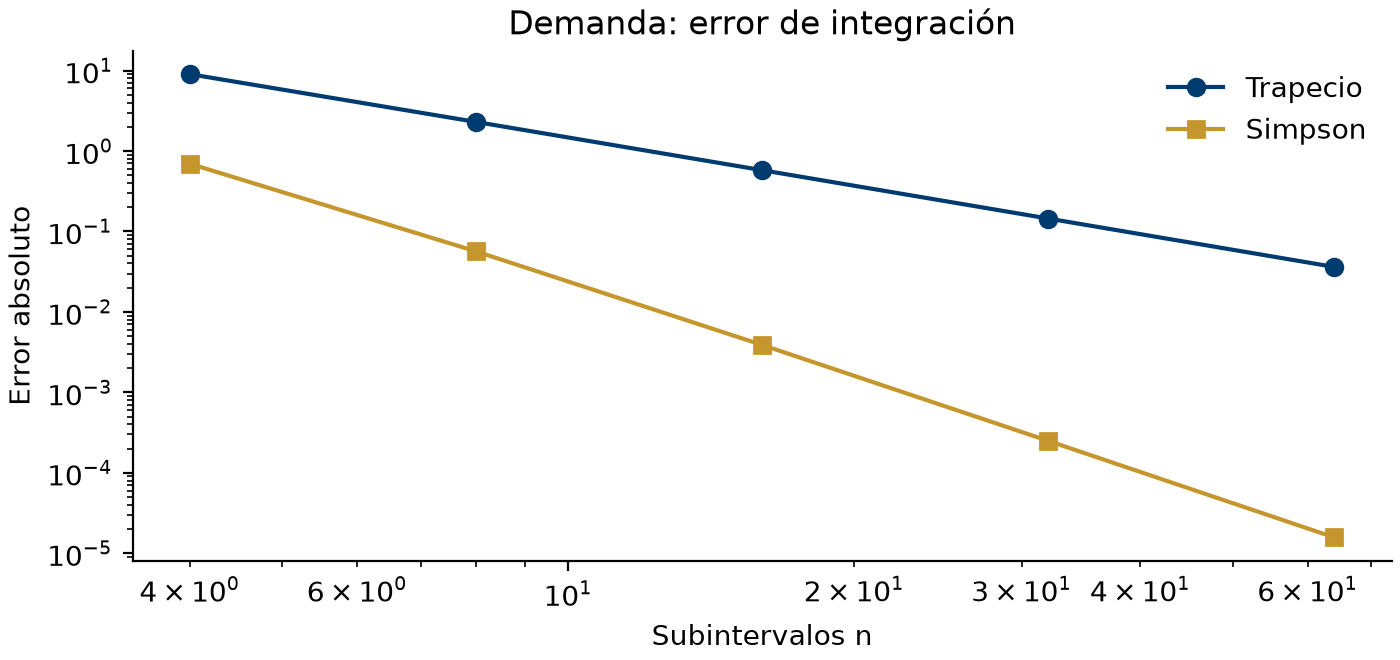
\includegraphics[height=.66\textheight]{figuras/integracion/convergencia.png}\end{center}
Al duplicar $n$, los errores se reducen aproximadamente por factores $4$ y $16$
cuando domina el término asintótico de trapecio y Simpson, respectivamente.
\end{frame}

\begin{frame}{Elección de la malla por una cota}
Para la demanda anterior,
\[p''(q)=\frac1{(1+q/10)^3},\qquad
p^{(4)}(q)=\frac{0.12}{(1+q/10)^5}.\]
En $[0,20]$, $M_2=1$ y $M_4=0.12$. Para exigir error $\leq\varepsilon$ basta
\[n\geq\sqrt{\frac{20^3M_2}{12\varepsilon}}\quad\text{(trapecio)},\qquad
n\geq\left(\frac{20^5M_4}{180\varepsilon}\right)^{1/4}\quad\text{(Simpson)}.\]
Con $\varepsilon=0.01$, son suficientes $n_T=259$ y $n_S=22$.
Son condiciones suficientes, no los menores valores posibles de $n$.
\end{frame}

\begin{frame}[fragile]{Implementación del trapecio}
\begin{lstlisting}
import numpy as np

def trapecio(f, a, b, n):
    if n < 1 or int(n) != n:
        raise ValueError("n debe ser entero positivo")
    n = int(n)
    x = np.linspace(a, b, n+1)
    y = f(x)
    h = (b-a)/n
    return h*(y[0]/2 + y[1:-1].sum() + y[-1]/2)
\end{lstlisting}
La función $f$ debe aceptar vectores; aquí se supone $a<b$ y valores finitos.
Cada evaluación usa $n+1$ nodos. El cuaderno incorpora estas comprobaciones.
\end{frame}

\begin{frame}[fragile]{Implementación de Simpson}
\begin{lstlisting}
def simpson_compuesto(f, a, b, n):
    if n < 2 or int(n) != n or n % 2:
        raise ValueError("n debe ser entero positivo y par")
    n = int(n)
    x = np.linspace(a, b, n+1)
    y = f(x)
    h = (b-a)/n
    return h/3*(y[0] + y[-1]
        + 4*y[1:-1:2].sum() + 2*y[2:-1:2].sum())
\end{lstlisting}
Verifique la exactitud sobre $1,x,x^2,x^3$ y compruebe que se rechace un $n$ impar.
\end{frame}

\begin{frame}[fragile]{Verificación con bibliotecas}
\begin{lstlisting}
from scipy.integrate import trapezoid, simpson, quad
p = lambda q: 50/(1+q/10)
x = np.linspace(0., 20., 17)  # 16 subintervalos
y = p(x)
T = trapezoid(y, x=x)
S = simpson(y, x=x)
valor, error_estimado = quad(p, 0., 20.)
\end{lstlisting}
\texttt{trapezoid} y \texttt{simpson} integran muestras.
\texttt{quad} evalúa una función y adapta la partición.
Su error devuelto es una estimación numérica, no una cota certificada universal.
\end{frame}

\begin{frame}{Refinamiento y error estimado}
Si $Q_h=I+Ch^p+o(h^p)$ y $Q_{h/2}=I+C(h/2)^p+o(h^p)$, entonces
\[|I-Q_{h/2}|\approx\frac{|Q_{h/2}-Q_h|}{2^p-1}.\]
Para trapecio usamos $p=2$ y divisor $3$; para Simpson, $p=4$ y divisor $15$.
\begin{block}{Alcance}
Es una estimación asintótica. Puede fallar con discontinuidades, singularidades,
oscilaciones no resueltas o errores de redondeo dominantes.
\end{block}
Un criterio de parada debe incluir tolerancia, máximo de refinamientos y motivo de salida.
\end{frame}

\begin{frame}{Ejemplo oscilatorio de las notas}
\[I=\int_1^3\frac{100}{x^2}\sin\left(\frac{10}{x}\right)\,dx
=10\left[\cos(10/3)-\cos(10)\right]\approx-1.426024756346.\]
El cambio $u=10/x$ permite auditar el resultado.
\begin{center}\begin{tabular}{rrr}\toprule
$n$&$S_n$&$I-S_n$\\\midrule
400&$-1.426024347714$&$-4.0863\times10^{-7}$\\
1000&$-1.426024745884$&$-1.0462\times10^{-8}$\\\bottomrule
\end{tabular}\end{center}
El segundo cálculo cumple una tolerancia absoluta $10^{-7}$.
\end{frame}

\begin{frame}{Actividad de cierre}
\begin{enumerate}
\item Calcule el excedente con $n=8,16,32$ y compare el costo de cada regla.
\item Justifique el signo del error del trapecio en este ejemplo.
\item Explique la diferencia entre una cota con derivadas, una estimación
por refinamiento y el error observado frente a una referencia exacta.
\end{enumerate}
\textquestiondown{}Qué información pierde una integración basada únicamente en una tabla de datos?
\end{frame}

\begin{frame}{Complemento: reglas abiertas}
Los nodos evitan los extremos:
\[x_j=a+(j+1)h,\quad j=0,\ldots,n,\qquad h=\frac{b-a}{n+2}.\]
Los pesos siguen siendo $\alpha_j=\int_a^b L_j(x)\,dx$.
Se conserva el principio de integrar el interpolante.
\begin{block}{Uso e hipótesis}
No evaluar en los extremos puede ser útil, pero las cotas clásicas siguen
requiriendo la regularidad indicada en todo el intervalo.
Una singularidad necesita un tratamiento específico.
\end{block}
\end{frame}

\begin{frame}{Punto medio y regla abierta de dos nodos}
Si $f\in C^2[a,b]$, para algún $\xi\in(a,b)$:
\[M(f)=(b-a)f\left(\frac{a+b}2\right),\qquad
I-M=\frac{(b-a)^3}{24}f''(\xi).\]
Con nodos $u=a+(b-a)/3$ y $v=a+2(b-a)/3$,
\[O_2(f)=\frac{b-a}{2}[f(u)+f(v)],\qquad
I-O_2=\frac{(b-a)^3}{36}f''(\xi).\]
Al componer paneles de ancho $H$, las cotas son
$(b-a)H^2M_2/24$ y $(b-a)H^2M_2/36$, respectivamente.
\end{frame}

\begin{frame}{Regla abierta de tres nodos}
Sean $u=a+(b-a)/4$, $c=(a+b)/2$ y $v=a+3(b-a)/4$.
\[O_3(f)=\frac{b-a}{3}[2f(u)-f(c)+2f(v)].\]
Si $f\in C^4[a,b]$, para algún $\xi\in(a,b)$,
\[I-O_3=\frac{7(b-a)^5}{23040}f^{(4)}(\xi).\]
Al componer paneles de ancho $H$,
\[|E|\leq\frac{7(b-a)H^4}{23040}\norm{f^{(4)}}_\infty.\]
Cada panel lleva el factor $H/3$. Los pesos suman $H$; esta verificación
permite detectar un coeficiente incorrecto.
\end{frame}

\begin{frame}{Tabla de Newton--Cotes cerrada}
\small
Con $n+1$ nodos equidistantes, los siguientes vectores se multiplican por $b-a$:
\begin{center}\begin{tabular}{clc}\toprule
$n$&Pesos normalizados&Grado exacto\\\midrule
1&$(1,1)/2$&1\\
2&$(1,4,1)/6$&3\\
3&$(1,3,3,1)/8$&3\\
4&$(7,32,12,32,7)/90$&5\\
5&$(19,75,50,50,75,19)/288$&5\\
6&$(41,216,27,272,27,216,41)/840$&7\\\bottomrule
\end{tabular}\end{center}
La fila $n=3$ corresponde a la regla $3/8$; la de $n=4$, a Boole.
Cada fila suma $1$. Para reglas de grado alto pueden aparecer pesos negativos:
la fórmula sigue teniendo sentido algebraico, pero puede amplificar perturbaciones.
\end{frame}

\begin{frame}{Exactitud y cotas para datos perturbados}
En Newton--Cotes cerrada, el grado de exactitud es $n$ si $n$ es impar
y $n+1$ si $n$ es par. En el segundo caso interviene la simetría.
Si cada valor de $f$ se perturba en $\delta_j$, con $|\delta_j|\leq\eta$,
\[|\Delta Q|=\left|\sum_j\alpha_j\delta_j\right|
\leq\eta\sum_j|\alpha_j|.\]
Con pesos no negativos, $\sum_j|\alpha_j|=b-a$.
Con pesos negativos, esa suma puede ser mayor.
\begin{block}{Elección práctica}
Refinar una regla de grado bajo permite controlar el error sin elevar
indefinidamente el grado de un único interpolante global.
\end{block}
\end{frame}

\begin{frame}{Núcleo de Peano y forma del error}
\small
\begin{thm}
Sea $E=I-Q$ una funcional de cuadratura exacta en $\PiN_{r-1}$.
Para $f\in C^r[a,b]$,
\[E(f)=\int_a^b K_r(t)f^{(r)}(t)\,dt,\qquad
K_r(t)=E_x\left(\frac{(x-t)_+^{r-1}}{(r-1)!}\right).\]
Por tanto, $|E(f)|\leq\norm{f^{(r)}}_\infty\int_a^b|K_r(t)|\,dt$.
Si $K_r$ conserva signo, existe $\xi\in(a,b)$ tal que
\[E(f)=C_r f^{(r)}(\xi),\qquad C_r=E(x^r)/r!.\]
\end{thm}
$(x-t)_+=\max\{x-t,0\}$. Esta condición de signo explica cuándo es válida
la forma del error con un único $\xi$.
\end{frame}

\begin{frame}{Errores generales de Newton--Cotes}
\small
Sea $\rho_n(x)=\prod_{j=0}^n(x-x_j)$ en una regla cerrada.
Si se cumple la condición de signo del núcleo de Peano:
\[
E_n(f)=\begin{cases}
\displaystyle\frac{f^{(n+1)}(\xi)}{(n+1)!}\int_a^b\rho_n(x)\,dx,&n\text{ impar},\\[2mm]
\displaystyle\frac{f^{(n+2)}(\xi)}{(n+2)!}\int_a^b x\rho_n(x)\,dx,&n\text{ par}.
\end{cases}\]
Se supone $f\in C^{n+1}$ o $C^{n+2}$, respectivamente.
Para nodos abiertos $x_j=a+(j+1)h$, la constante es
\[\frac{h^{n+2}}{(n+1)!}\int_{-1}^{n+1}\prod_{j=0}^n(t-j)\,dt\quad(n\text{ impar}),\]
y para $n$ par se reemplaza por
$\frac{h^{n+3}}{(n+2)!}\int_{-1}^{n+1}t\prod_{j=0}^n(t-j)\,dt$.
Se aplica la hipótesis de signo; la cota integral anterior vale sin extraer $\xi$.
\end{frame}

\begin{frame}{Fuentes y continuación}
\small
\begin{itemize}
\item Material del curso: \texttt{unidadinteup.tex}, \texttt{unidadinte.tex} y capítulo 7 de las notas.
\item \href{https://dlmf.nist.gov/3.5}{NIST DLMF, sección 3.5: cuadratura y fórmulas de error}.
\item \href{https://www-users.cse.umn.edu/~arnold/597.00-01/nabook.pdf}{D. N. Arnold: \emph{A Concise Introduction to Numerical Analysis}},
capítulo 2, sección 2: teorema del núcleo de Peano.
\item \href{https://docs.scipy.org/doc/scipy/reference/generated/scipy.integrate.simpson.html}{SciPy: simpson}
\quad\href{https://docs.scipy.org/doc/scipy/reference/generated/scipy.integrate.quad.html}{SciPy: quad}.
\end{itemize}
La siguiente clase permite elegir los nodos para aumentar la exactitud:
cuadratura de Gauss. El complemento de integración doble se conserva allí.
\end{frame}

\end{document}
